\documentclass[graphics]{beamer}

\usepackage{graphicx}
\usepackage{verbatim}
\usepackage{wrapfig}
\useoutertheme{shadow}
%\usecolortheme{orchid}
\usecolortheme{seahorse}


% math commands
\newcommand{\be}{\begin{eqnarray}}
\newcommand{\ee}{\end{eqnarray}}
\newcommand{\beq}{\begin{equation}}
\newcommand{\eeq}{\end{equation}}
\def\simless{\mathbin{\lower 3pt\hbox
      {$\rlap{\raise 5pt\hbox{$\char'074$}}\mathchar"7218$}}}
\def\simgreat{\mathbin{\lower 3pt\hbox
      {$\rlap{\raise 5pt\hbox{$\char'076$}}\mathchar"7218$}}} %> or of order

% variables

\def\toonscale{0.45}
\def\mboxy#1{\mbox{\small #1}}


\begin{comment}
\AtBeginSection[]{
  \frame{
    \frametitle{Outline}
    \tableofcontents[currentsection]
  }
}
\end{comment}

\title{Classical Mechanics, Quantum Mechanics, Quantum Cosmology: new view on the universe
}
%\subtitle{interim update}
\author[U. Pen]{Ue-Li Pen (ASIAA and CITA), Dylan Jow (CITA), Job
  Feldbrugge (Edinburgh), TF Jiang (NYCU)
}
\date{January 18, 2023}


\begin{document}

%\section*{Introduction}
\section{Lenses}

\begin{comment}
  \subsection{Outline}

  \frame{
    \frametitle{Outline}
    \tableofcontents
  }
\end{comment}

\frame{\maketitle}


\frame{
\frametitle{Coherent Diffraction}
\begin{itemize}
\item using the full wave nature of light to probe matter:
\item X-ray Crystallography (van Laue, Nobel 1914)
\item Maser (Townes+, Nobel 1964)
\item Laser mapping, holography (Gabor, Nobel 1971)
\item Aperture Synthesis (Ryle, Nobel 1974)
\item Synchrotron Radiation Sources (Walker+Ramakrishnan, Nobel
  Chemistry 1997)
\end{itemize}
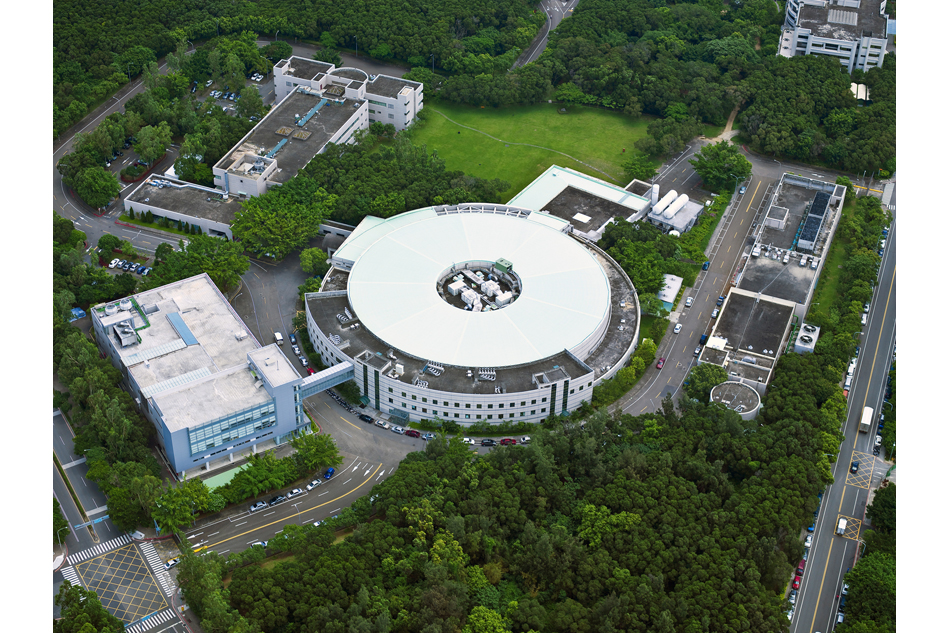
\includegraphics[width=2.3in]{Figures/nsrrc.png}
}



\frame{
\frametitle{Ptychography}
\begin{itemize}
\item (medical) X-ray imaging resolution $\sim$ mm
\item (phase retrieval ptychography) SRS coherent imaging resolution
  $\sim$ nm, million X more precise!
\item illustrates optics-free coherent image reconstruction
\end{itemize}
%\vspace{-0.5in}
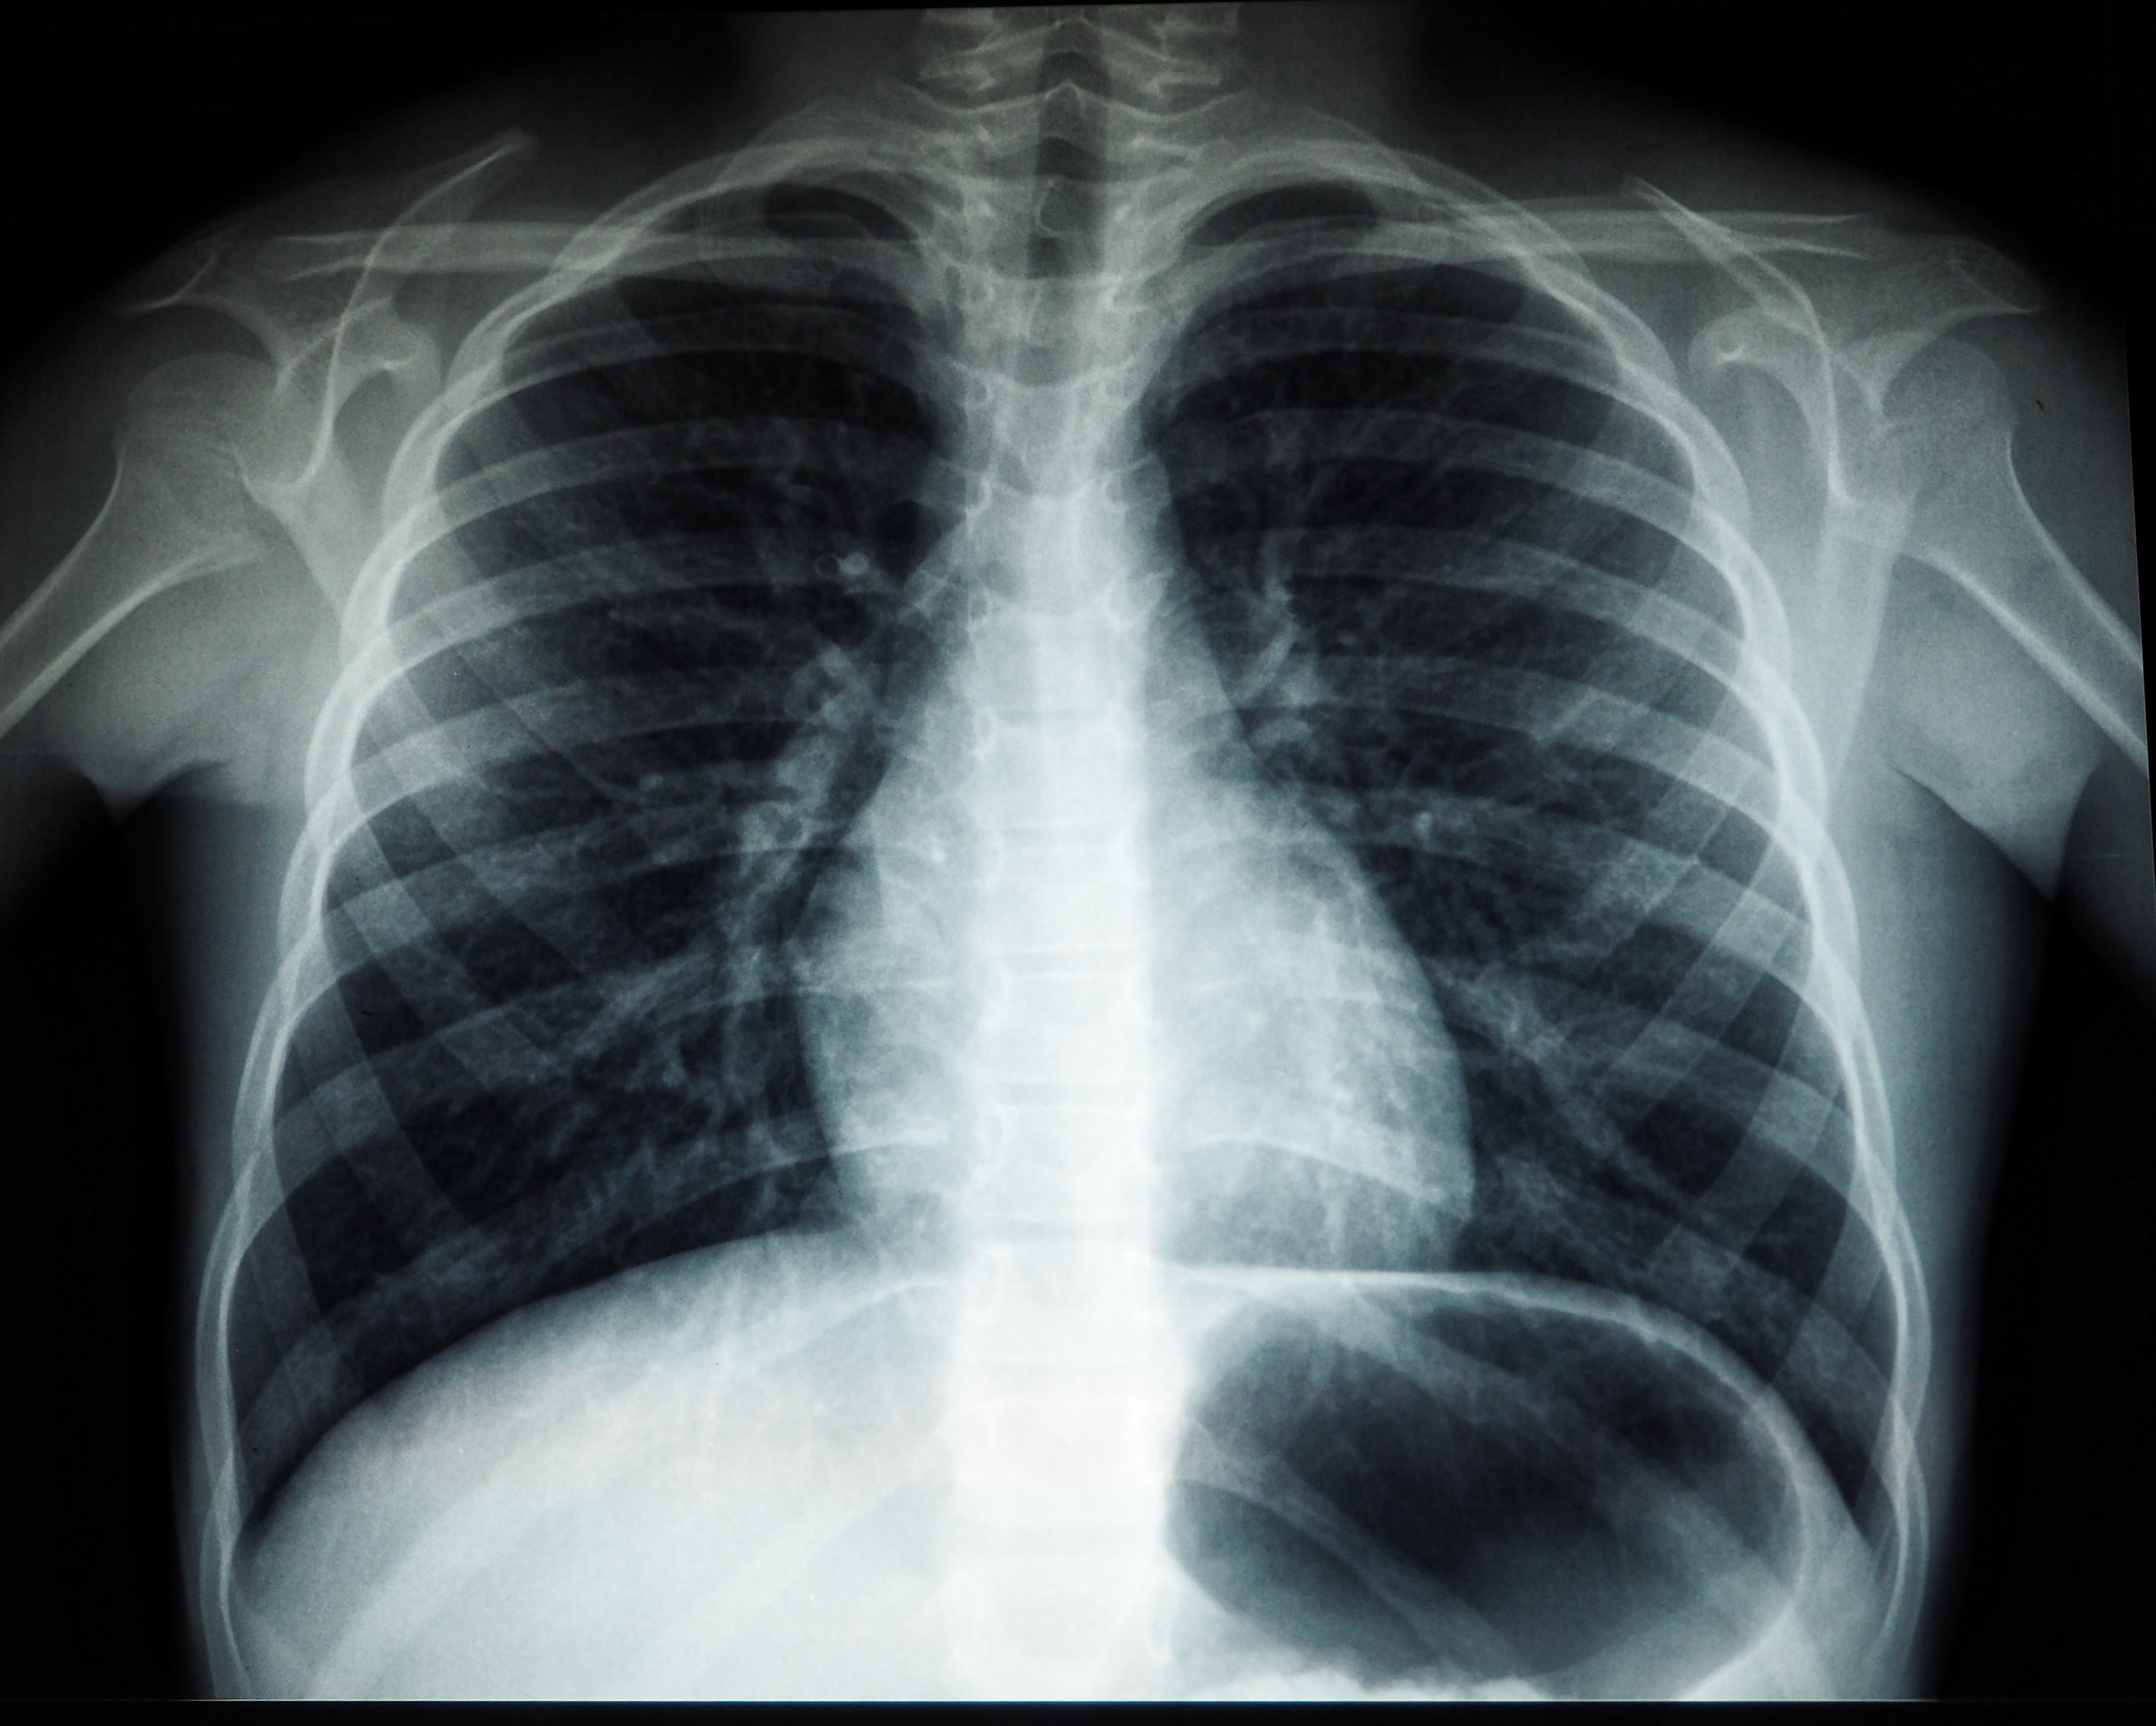
\includegraphics[width=1.5in]{Figures/xray.jpg}
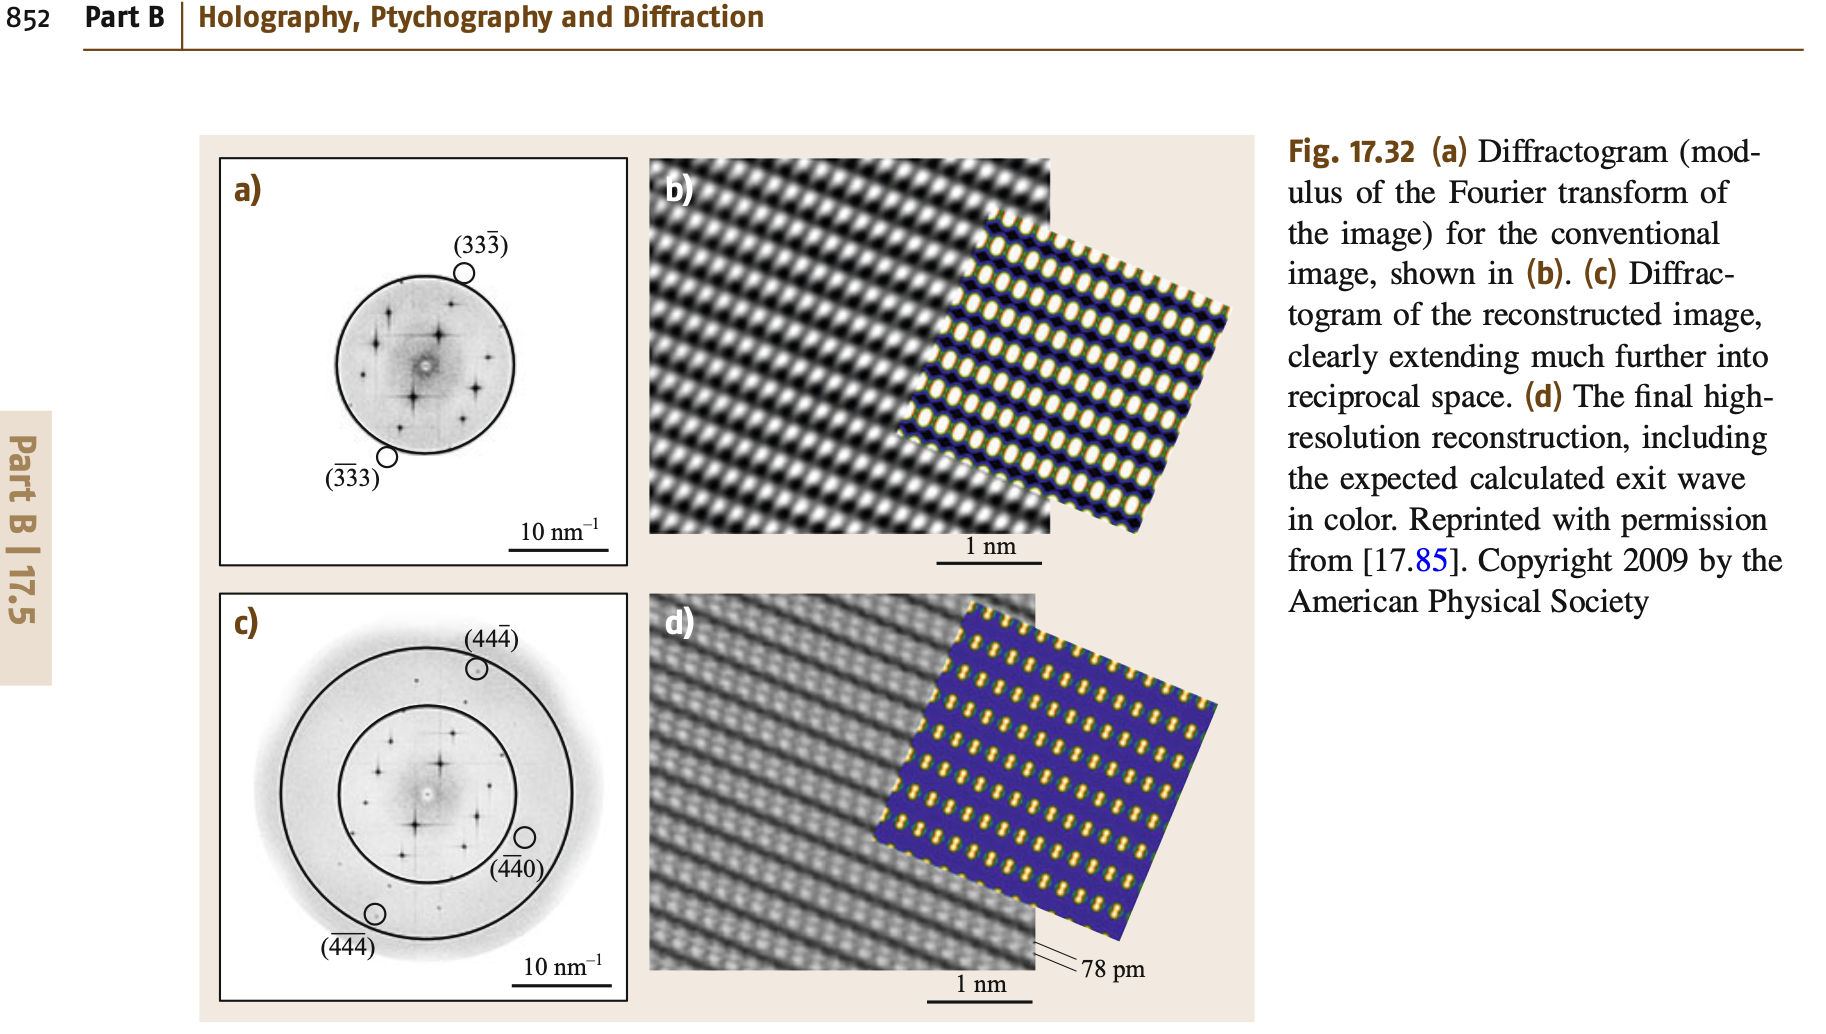
\includegraphics[width=2.75in]{Figures/ptychography.png}

{\tiny (Hawkes/Spence 2019)}
}

\frame{
\frametitle{Coherent Astrophysics}
\begin{itemize}
\item only two known sources of extragalactic coherent waves:
\item Gravitational Waves
\item Fast Radio Bursts
\item Coherent probe of space time: gravitational and plasma lensing
\end{itemize}
%\vspace{-0.5in}
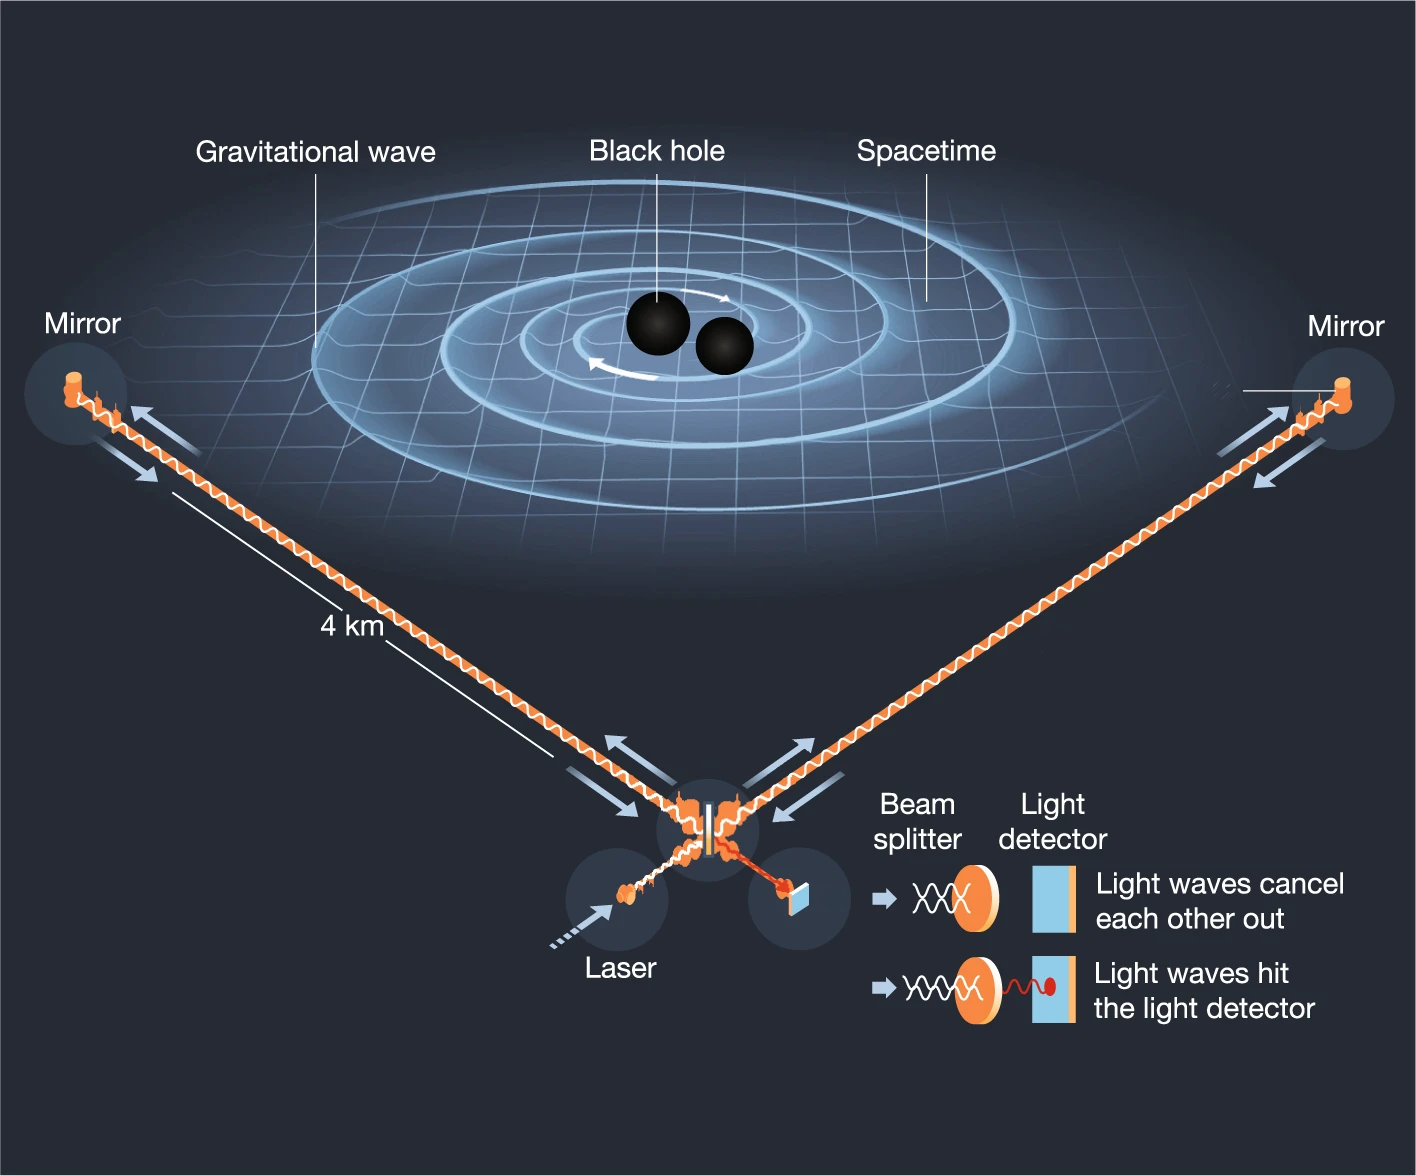
\includegraphics[width=1.9in]{Figures/GW.png}
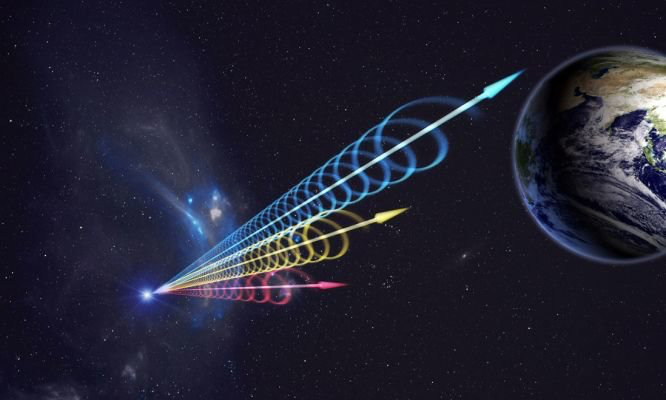
\includegraphics[width=2.3in]{Figures/FRB.png}
}


\frame{
\frametitle{Cosmic Ptychography}
\begin{itemize}
\item radio scintillation
\item VLBI through multiple telescopes
\end{itemize}
%\vspace{-0.5in}
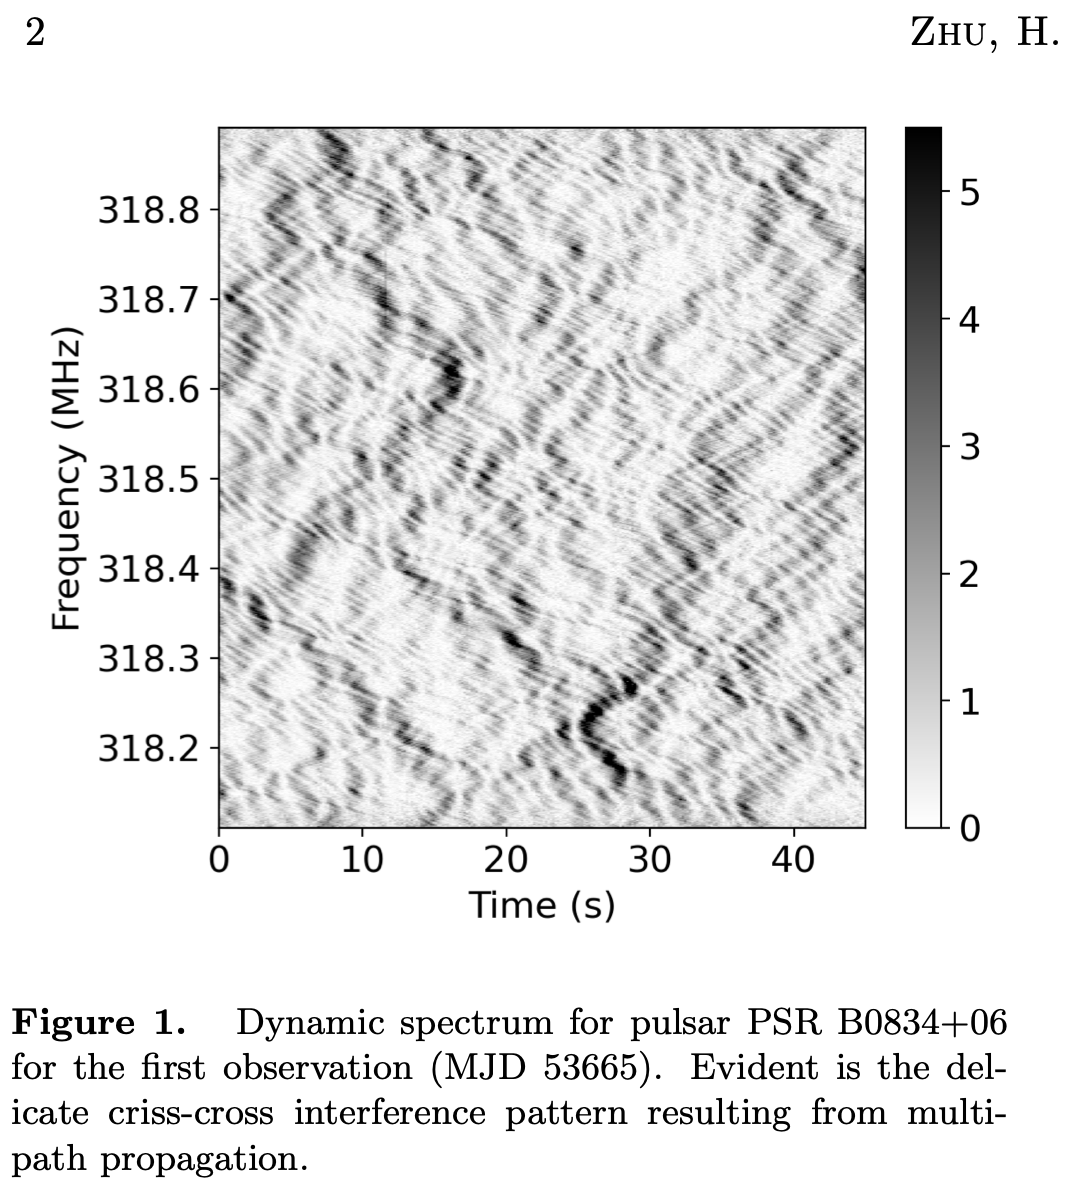
\includegraphics[width=2.2in]{Figures/b0834.png}
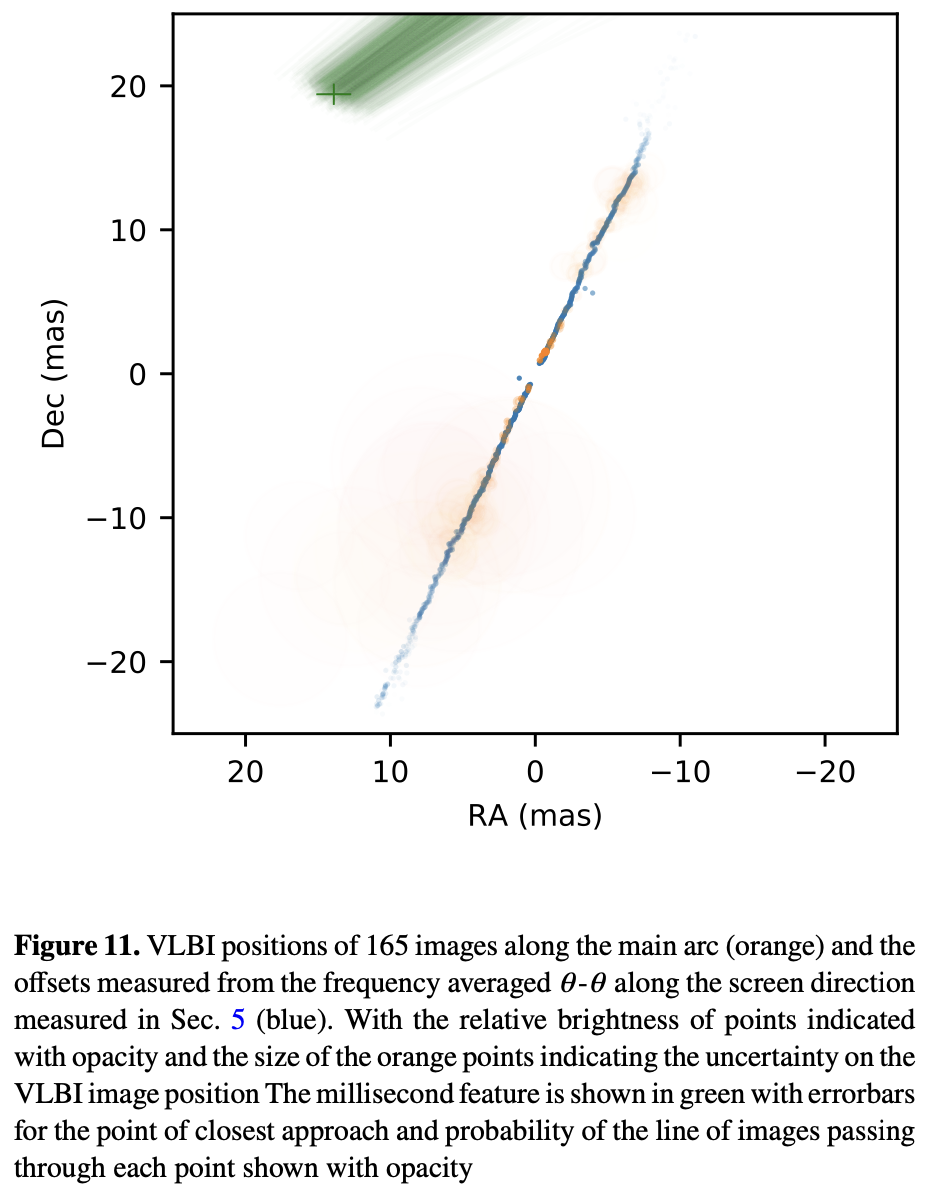
\includegraphics[width=2.1in]{Figures/vlbi.png}
}


  \frame{
    \frametitle{Wave Theory Picture}
    \begin{itemize}
        \item geometric optics and classical mechanics are intuitive
        \item wave optics and QM are abstract
        \item inverse problem infinitely harder for wave problems?
    \end{itemize}
  }


  \frame{
\vspace{-0.25in}
    \frametitle{Fermat's Principle}
    \begin{itemize}
        \item light takes shortest path. Why?
        \item Huygen's principle: light takes all paths
        \item Kirchoff/Feynmann path integral
        \item stationary phase dominates
        \item classical equation of motion: extremal paths, independent of wavelength
\vspace{-0.85in}\hspace{2.5in}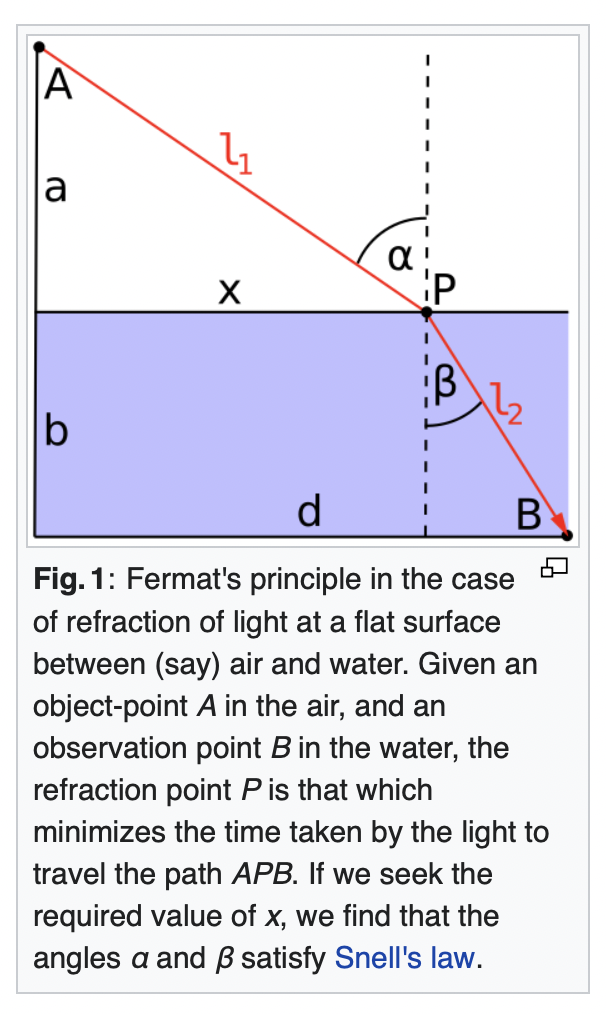
\includegraphics[width=1.3in]{Figures/fermat.png}
    \end{itemize}
  }




  \frame{
\vspace{-0.25in}
    \frametitle{Huygen's Principle: Path Integral}
    \begin{itemize}
        \item $A(\mu)=\int e^{i S(\theta,\mu)} d\theta$ 
        \item $S=\nu [(\theta-\mu)^2+\Psi(\theta)]$
        \item Highly oscillatory integral, even for $\Psi=0$
        \item Stationary phase points: $\partial_\theta S=0$ leads to (complex)
          Eikonal images $\theta_i$.
        \item flux/phase through curvature expansion (known as {\it
            steepest descent}): exact as $\nu \rightarrow \infty$
        \item Geometric limit considers only {\it Real} solutions $\theta_i$ and
      gives up phase
          information (length of trajectory)
        \item Geometric optics applicable at short wavelengths for
          extended sources
          (e.g. optical gravitational lensing of finite size sources,
          stars)     
    \end{itemize}
  }



  \frame{
\vspace{-0.5in}
    \frametitle{Picard-Lefschetz Theory}
    \begin{itemize}
    \item descend integral along real line along Morse function Im(S)
    \item contour deforms into finite number of Thimbles of constant
      phase with maximum at saddle point (extrema $dS=0$)
    \item correctly identifies relevant saddle points
    \item resolves numerical challenges of oscillatory integral
    \item complex analysis works in multiple variables
    \item elevates concept of ``image'' deep into wave optics
    \item multiple public implementations (Feldbrugge+, Jow+)
    \end{itemize}
  }



  \frame{
\vspace{-0.5in}
    \frametitle{Picard-Lefschetz Theory}

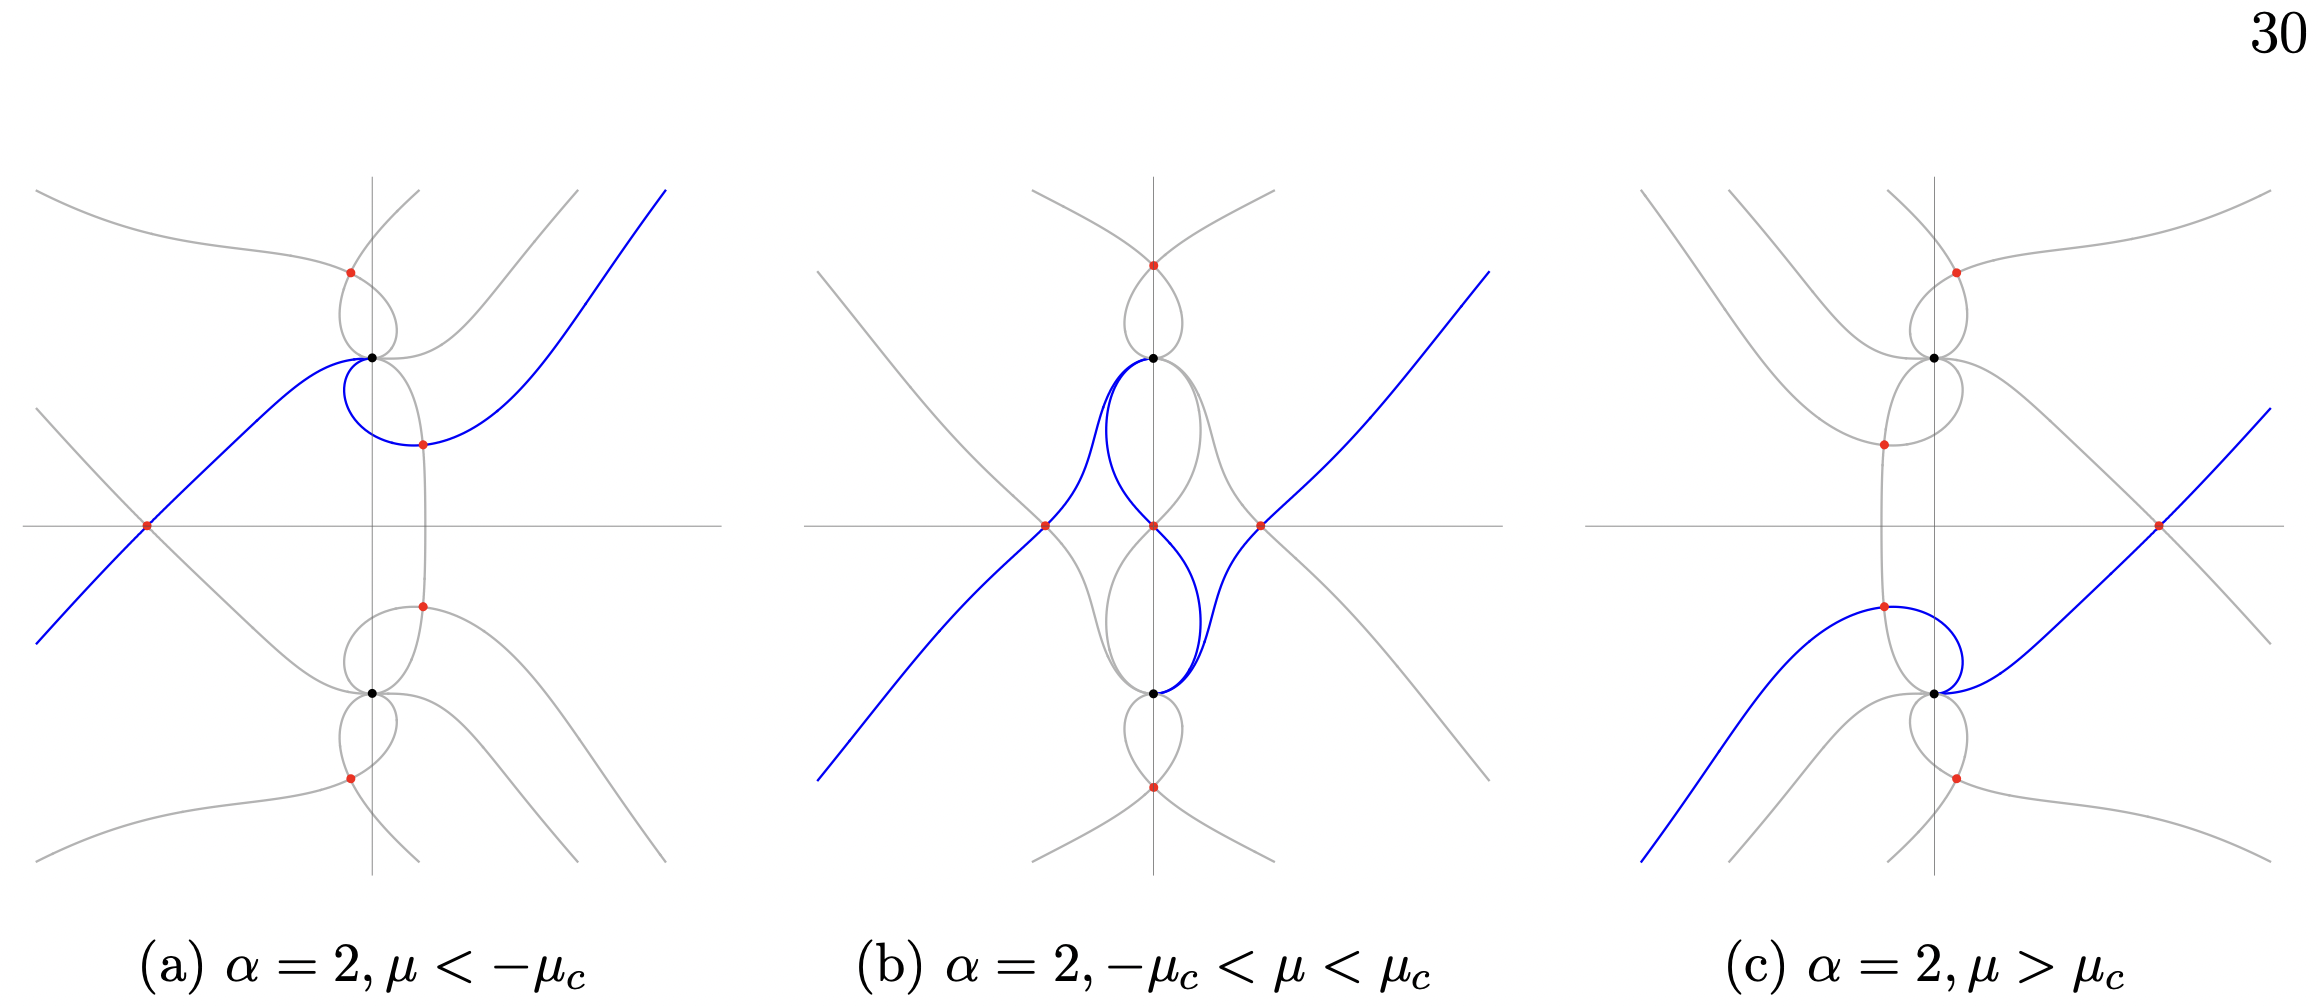
\includegraphics[width=4.5in]{Figures/thimbles.png}

Feldbrugge+2019
  }


  \frame{
\vspace{-0.5in}
    \frametitle{Imaginary classical paths}
    \begin{itemize}
    \item PL interpretation: oscillatory integral is sum over thimbles
    \item each thimble has exactly one stationary point (maxima, classical path)
    \item path integral is sum over thimbles
    \item eikonal limit is quadratic expansion at maxima (WKB for
      imaginary images)
    \item alternative interpretation of quantum mechanics from
      classical mechanics:
    \item sum over real and imaginary classical paths
    \item Turok 2014, Cherman+ 2014, Mou+ 2019
    \end{itemize}
  }

  \frame{
\vspace{-0.5in}
    \frametitle{New Observables}
    \begin{itemize}
    \item for coherent sources: FRBs, pulsars
    \item weak lensing: imaginary image allows time delay measurement (Jow+21)
    \item strong lensing: delay measurements enable measurement of
      co-linearity (Jow++21)
    \item microlensing: instant time delay, planets (Jow+20)
    \item macrolensing: potentially nano-second delay -- universe
      expands!  Dark energy, etc (Wucknitz+21)
    \item dimensionless strain cm/Gigalightyears $h\sim \Delta t/t \sim 10^{-26}$:
      competitive with LIGO, etc
    \end{itemize}
  }




  \frame{
\vspace{-0.5in}
    \frametitle{Lorenzian Quantum Cosmology}
    \begin{itemize}
    \item Feldbrugge, Lehners \& Turok 2017
    \item Quantize Feynmann path integral instead of wave equation
    \item PL, Cauchy's theorem allow deformation of paths into complex plane
    \item minisuperspace: allow imaginary paths (scale factor)
    \item PL Semi-classical limit: dominant paths
    \item CPT universe, bounce, etc (Boyle, Finn, Turok 2018)
    \end{itemize}
  }



  \frame{
\vspace{-0.5in}
    \frametitle{Discussion}
    \begin{itemize}
    \item Eikonal effects applicable to compact radio sources,
      e.g. FRBs, pulsars
    \item full wave
effect dominates for long wavelengths as Fresnel scale is bigger then Einstein radius
    \item down to planet size
    \item gravitational waves:  LIGO, LISA, PTA
    \end{itemize}
  }


\frame{
    \frametitle{BURSTT}
Bustling Universe Radio Telescope Taiwan: collaboration of ASIAA, NTU,
NTHU, NCHU for all sky FRB radio array
     \hspace{-0.5in}
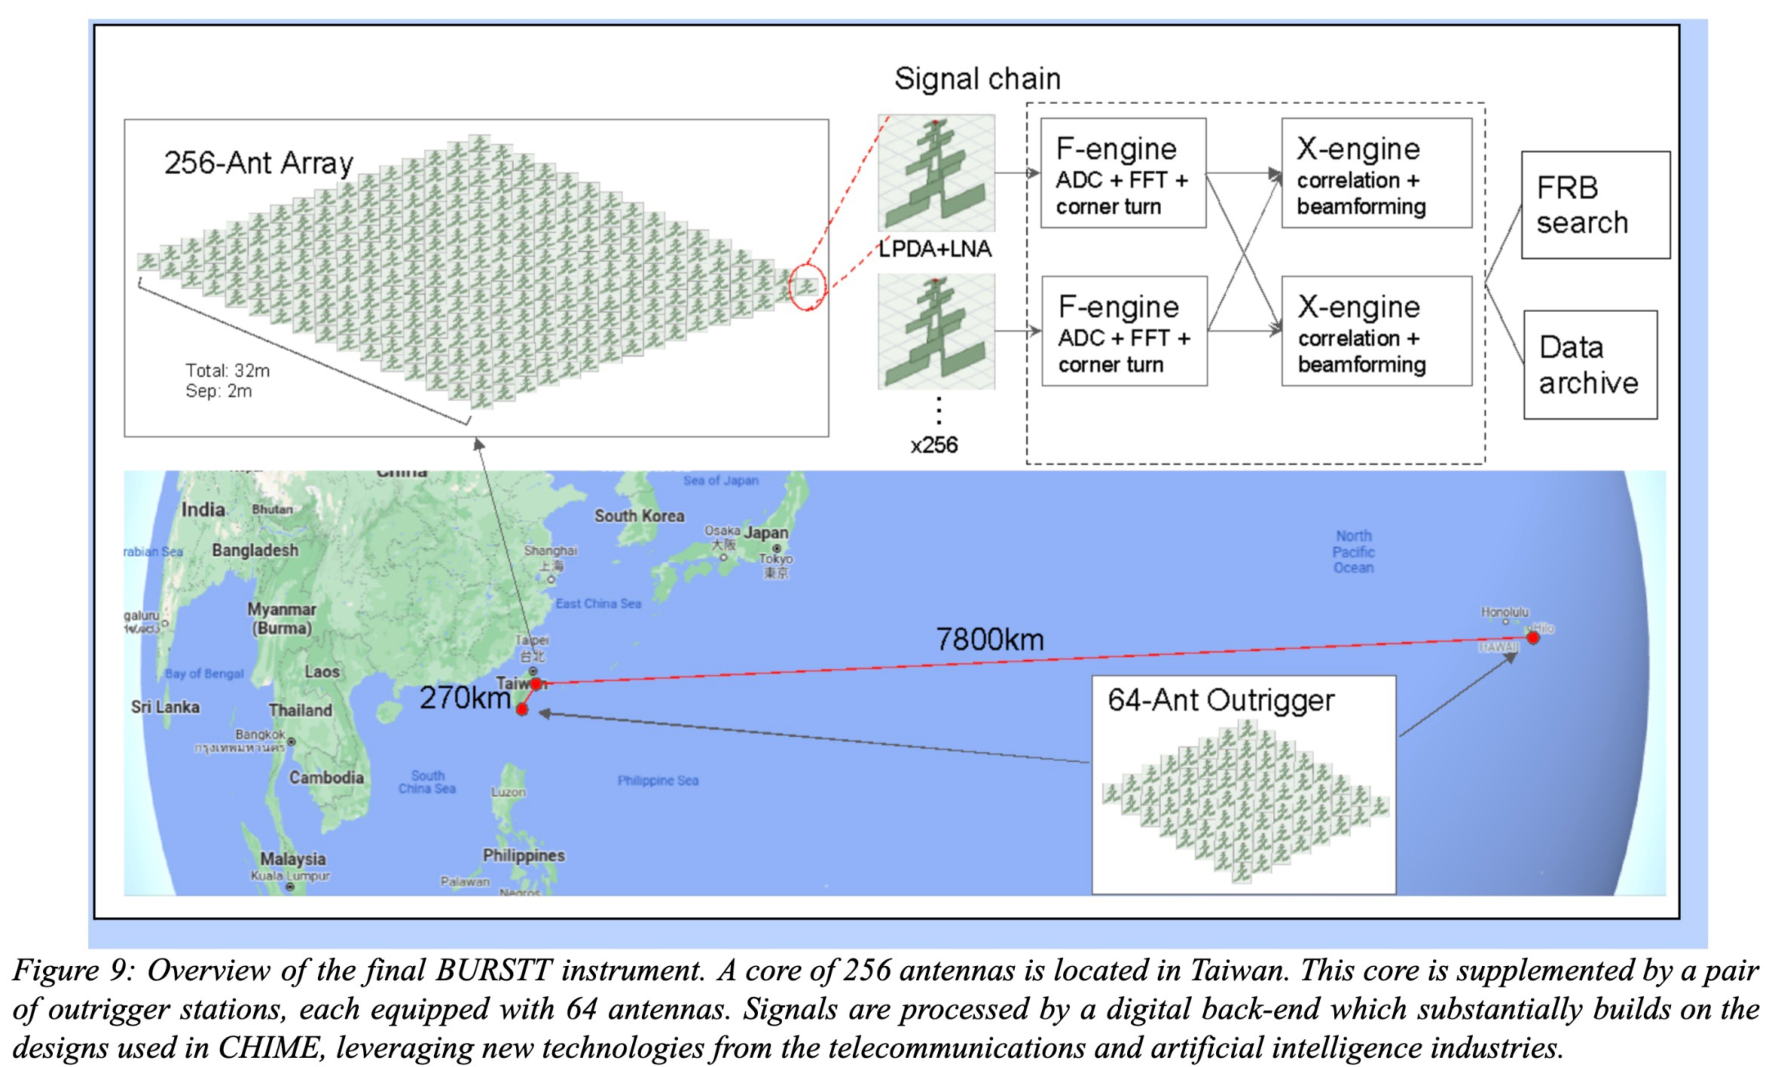
\includegraphics[width=0.55\textwidth]{Figures/BURSTT.pdf}
\includegraphics[width=0.45\textwidth]{Figures/fushanplatform.jpeg}
}

\frame{
\frametitle{What is filling the universe?}
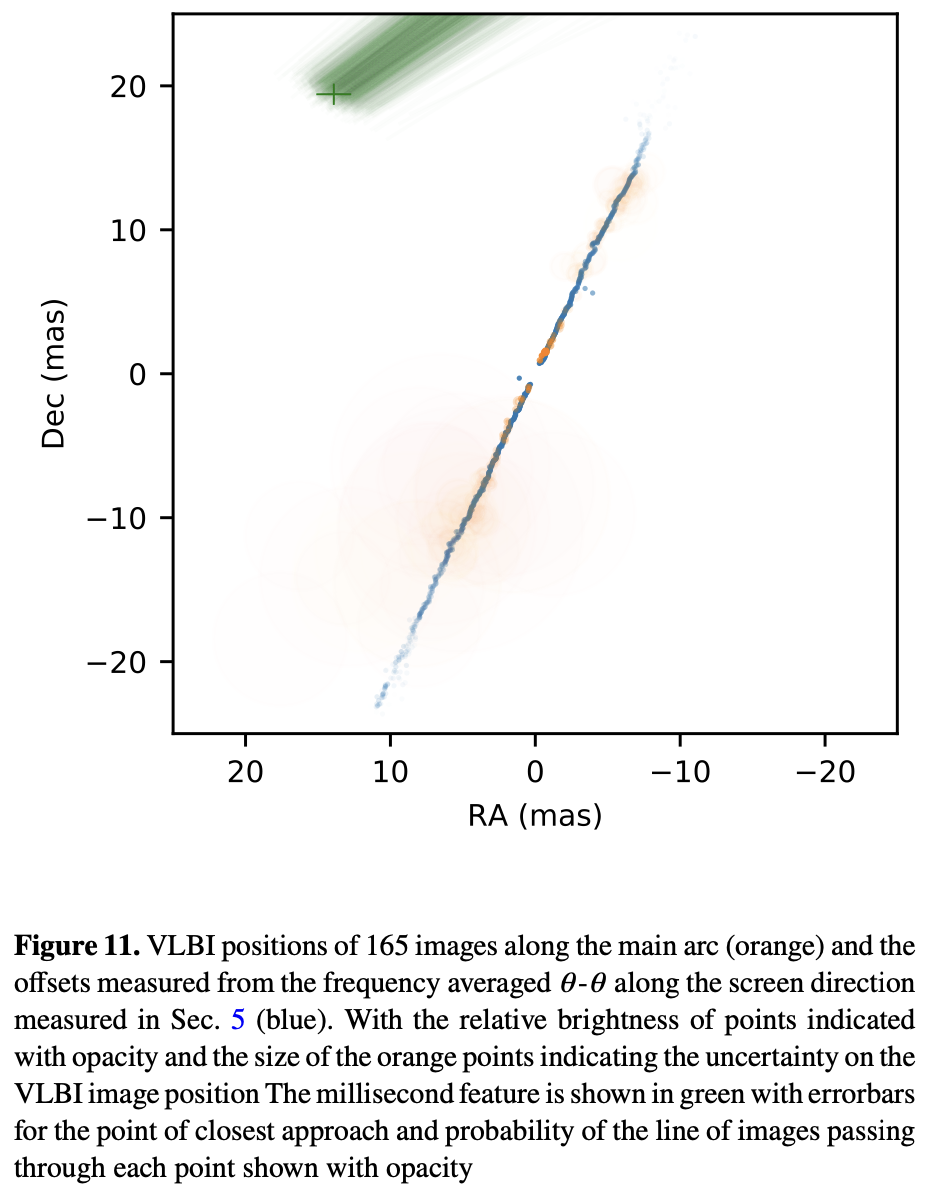
\includegraphics[width=3.2in]{Figures/vlbi.png}

}

\frame{
\frametitle{1-D lenses}
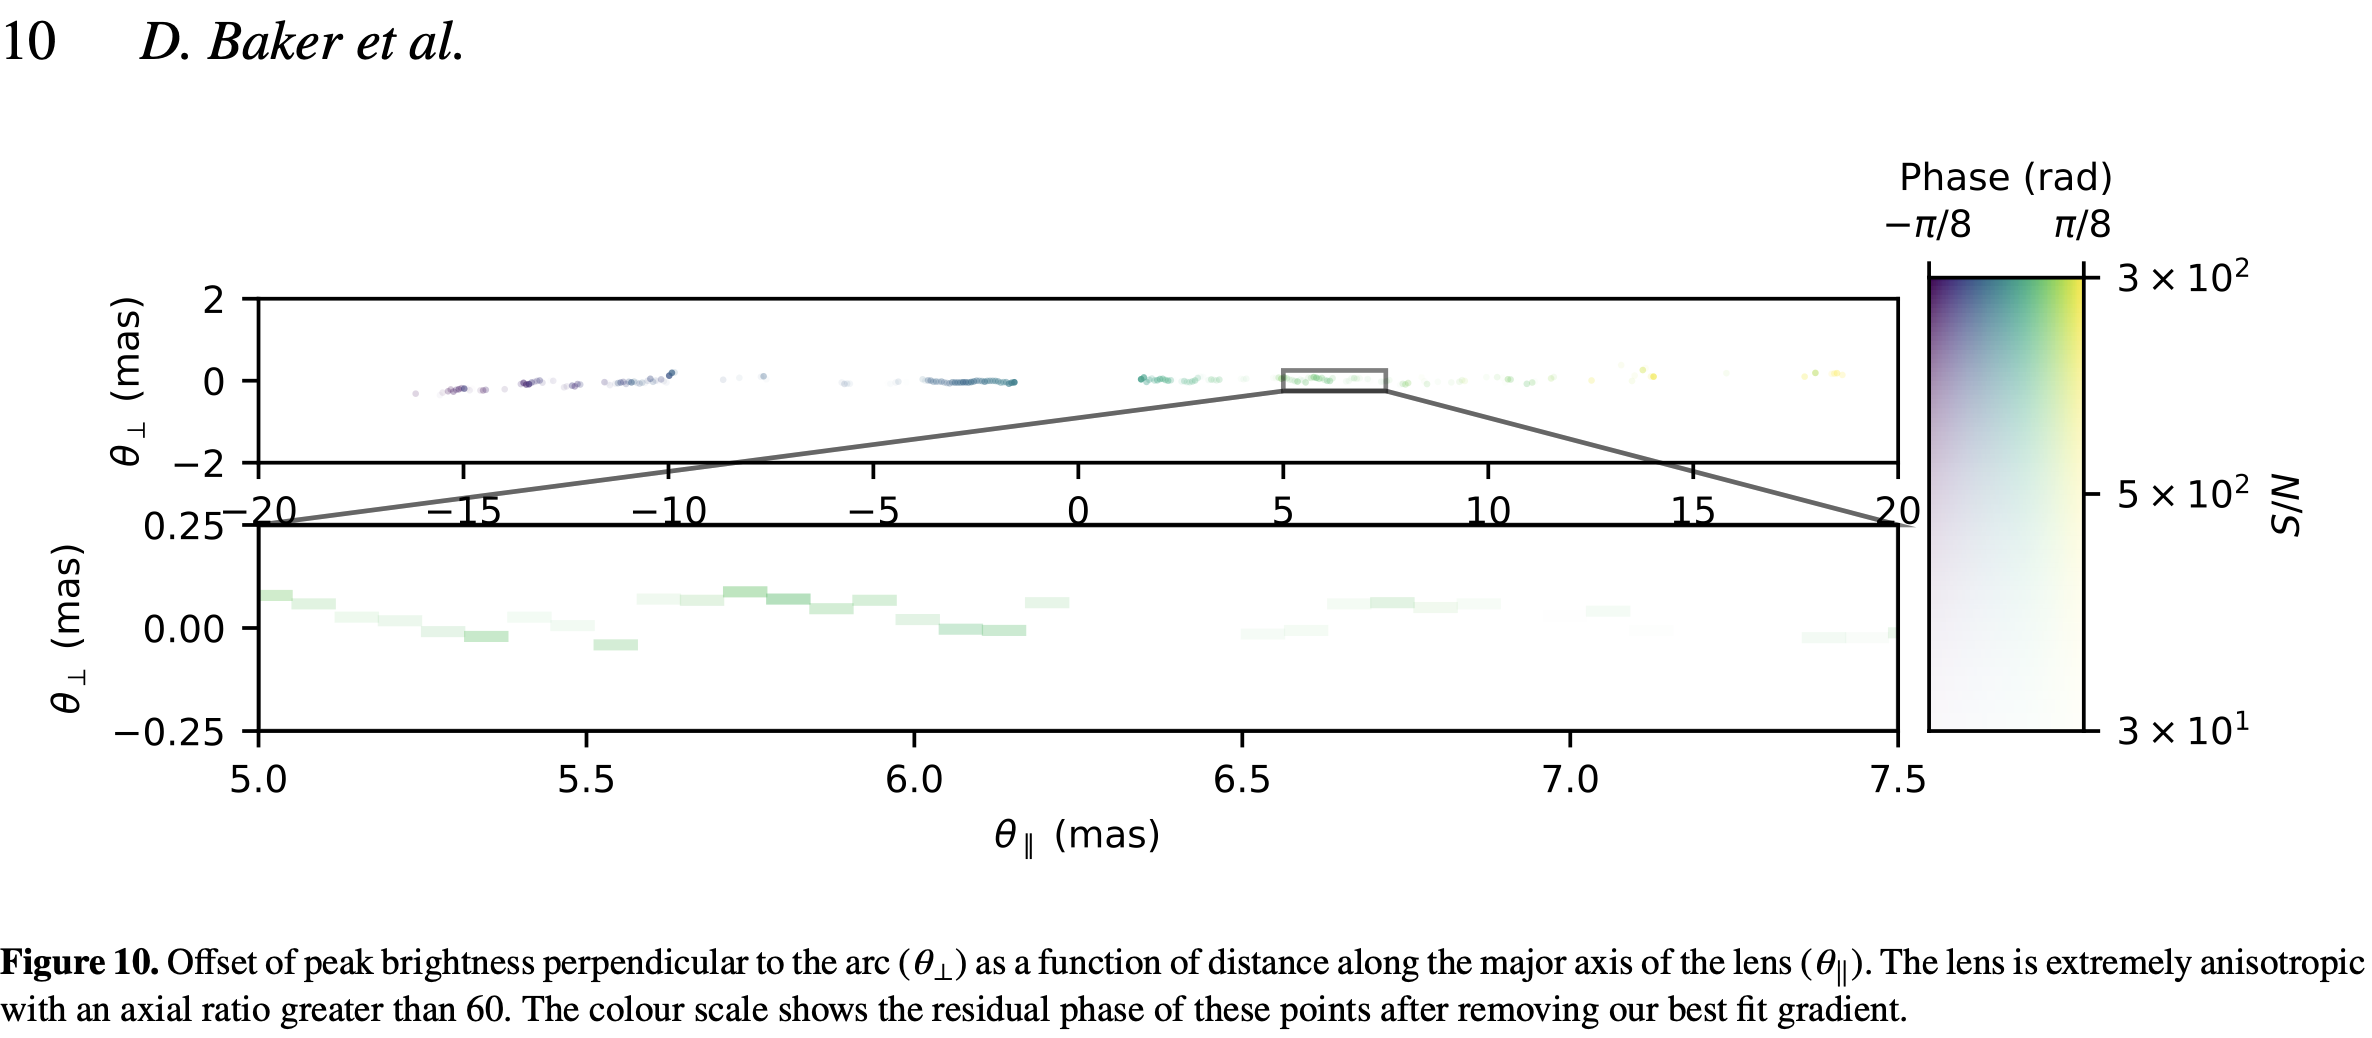
\includegraphics[width=4.5in]{Figures/theta-theta.png}
}

\frame{
    \frametitle{Magnetic Domain Boundaries?}
\begin{itemize}
\item universe filled with highly conductive magnetized plasma
\item local regions minimize energy by aligning fields, in analogy
  with ferromagnet
\item domain boundary between regions of differing field angles
\item {\it domain walls} dominate radio plasma lensing at projected
  caustics (Jow, ULP,+23)
\end{itemize}
}


\frame{
\frametitle{Domain Walls}
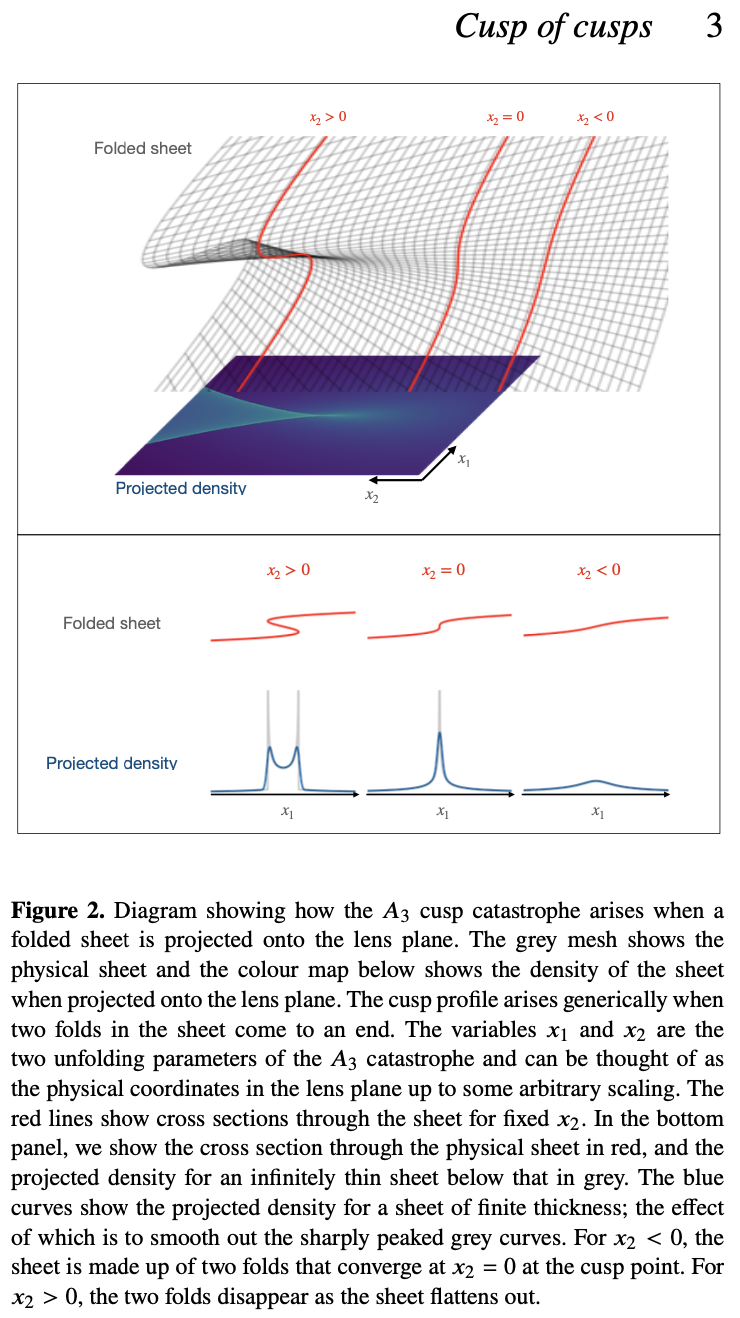
\includegraphics[width=4.5in]{Figures/cusp.png}
}

  \frame{
%\vspace{-0.5in}
    \frametitle{Conclusions}
    \begin{itemize}
    \item Cosmic application of holographic/ptychographic techniques
      with new coherent sources: FRBs, GWs, pulsars
    \item unprecedented precision probes of space yielding puzzling results
    \item new wave optics problems, complex images
    \item Picard-Lefschetz theory provides alternative interpretation
      of optics, quantum mechanics: imaginary positions and trajectories
    \item wave optics changes nature of astrophysical observables: Coherent FRB
      radiation one of the potentially most
      precise measurements in physics. 
    \item new tool to compute quantum gravity, bypassing historical conceptual barriers.
    \end{itemize}
  }

\end{document}
